
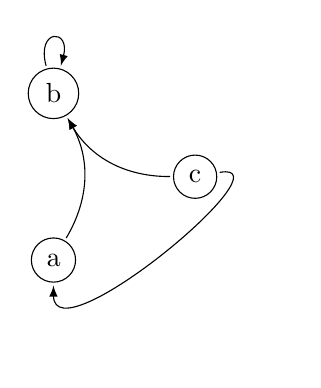
\begin{tikzpicture}[>=latex,line join=bevel,shorten >=1pt,shorten <=1pt]
%%
\node (a) at (19bp,19bp) [draw,circle] {a};
  \node (c) at (70bp,49bp) [draw,circle] {c};
  \node (b) at (19bp,79bp) [draw,circle] {b};
  \draw [->] (c) to[out=10,in=-90] (a);
  \draw [->] (a) to[bend right] (b);
  \draw [->] (c) to[bend left] (b);
  \draw [->] (b) to[loop above] (b);
%
\end{tikzpicture}
